\documentclass[11pt]{article}
\usepackage{graphicx}
\graphicspath{ {./} }
\usepackage{booktabs}
\usepackage[a4paper, margin=1in]{geometry}
\usepackage{amsmath}
\usepackage{float}

\renewcommand\thesubsection{(\roman{subsection})}
\makeatletter
\@addtoreset{subsection}{section}
\makeatother

\title{\vspace{-2cm}AERO 516: Quals Review\vspace{-1.0cm}}
\renewcommand\thesubsection{\thesection.\arabic{subsection}}

\begin{document}
    \maketitle

    \section{Basic Concepts}
    \subsection{Properties of Composites}
    \begin{itemize}
        \item{Out-of-plane properties are generally very weak}
        \item{Much manufacturing variability}
        \item{Greatest specific stiffness of any material}
    \end{itemize}

    \begin{figure}[H]
        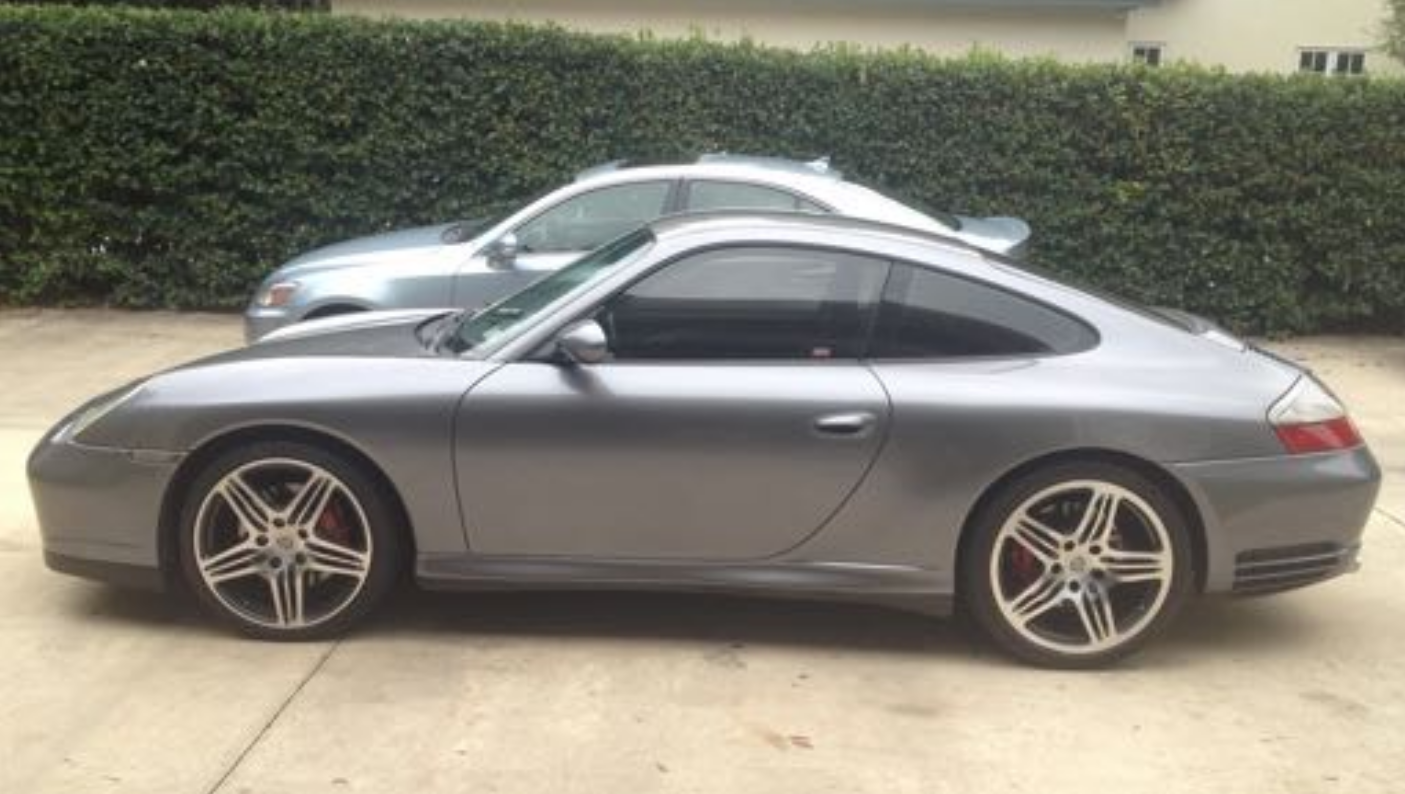
\includegraphics[width=6cm]{porsche}\centering
        \caption{Sodano's whip}
        \label{fig:1}
    \end{figure}

    \subsection{Fiber Notes}
    \begin{itemize}
        \item{Types: glass, carbon, SiC, boron, polymer}
        \item{Tow is the number of filaments}
        \item{Carbon fiber: 225-500 GPa modulus, 3400-6400 MPa strength}
    \end{itemize}

    \section{Lamina Stress-Strain Relationships}
    \subsection{Stress-Strain Basics}

    \begin{figure}[H]
        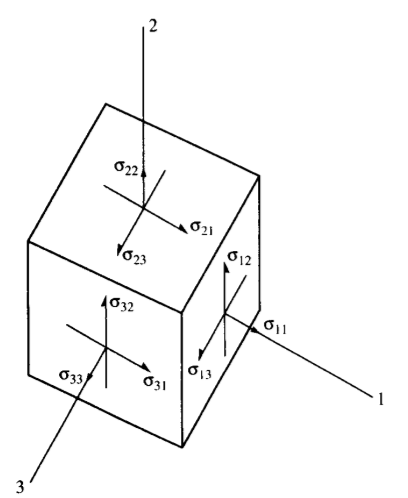
\includegraphics[width=6cm]{3D_stress_state}\centering
        \caption{3D stress representation}
        \label{fig:2}
    \end{figure}

    \begin{itemize}
        \item{$\{ \pmb{\sigma} \} = [\mathbf{C}] \{ \pmb{\epsilon} \}, C$ is the stiffness matrix}
        \item{$\{ \pmb{\epsilon} \} = [\mathbf{S}] \{ \pmb{\sigma} \}, S$ is the compliance matrix}
        \item{$\mathbf{S} = \mathbf{C}^{-1}$}
        \item{Stress and strain can be averaged over a specimen, such as:}
        \item{$ \bar{\sigma_i} = \int_V{\sigma_i}dv/V$ and $ \bar{\epsilon} = \int_V{\epsilon_i}dv/V$}
        \item{$ \bar{\sigma_i} = C_{ij} \bar{\epsilon_j}$ and $ \bar{\epsilon} = S_{ij} \bar{\sigma}$}
        \item{$ W = \frac{1}{2} C_{ij} \epsilon_i \epsilon_j$}
        \item{S, the compliance matrix, contains the simpler terms in regards to engineering terms}
    \end{itemize}

    \begin{table}[]
        \def\arraystretch{1.2}
        \centering
        \caption{Elastic coeffs}
        \label{my-label}
        \begin{tabular}{lll}
            Material and coord sys   & \# non-zero coeffs & \# ind coeffs \\ \hline
            3D aniso                 & 36                 & 21                \\
            3D gen ortho (non-princ) & 36                 & 9                 \\
            3D special ortho (princ) & 12                 & 9                 \\
            3D transversely iso      & 12                 & 5                 \\
            3D iso                   & 12                 & 2                 \\
            2D aniso                 & 9                  & 6                 \\
            2D gen ortho             & 9                  & 4                 \\
            2D special ortho (princ) & 5                  & 4                 \\
            2D square sym            & 5                  & 3                 \\
            2D iso                   & 5                  & 2                
        \end{tabular}
    \end{table}

    TODO: flesh this out, include 6x6 for special cases


    \subsection{Generally Orthotropic Lamina}



    \section{Effective Moduli of a Continuous Fiber-Reinforced Lamina}

    \subsection{Elementary Mechanics of Materials}

    \subsection{Improved Mechanics of Materials}

    \subsection{Micromechanics}

    \section{Strength of a Lamina}

    \subsection{Maximum Strength}

    \subsection{Maximum Stress}

    \subsection{Maximum Strain}

    \section{Analysis of Laminates}

    \subsection{Basics}

    \subsection{Classical Lamination Theory}

    \subsubsection{Assumptions}

    \subsubsection{Definitions}

    \subsubsection{Special Properties}

    \subsection{Laminate-Force Relations}

    \subsubsection{Determining Strain}

    \subsubsection{Determining Engineering Constants}

    \subsection{Hygrothermal Effects}





    \section{Previous Qual Questions}

    TODO: Add previous qual questions, esp. written on Dave's sheet

\end{document}